\documentclass[11pt,a4paper]{article}

\usepackage[T1]{fontenc}
\usepackage[utf8]{inputenc}
\usepackage{mathpazo}
\linespread{1.05}
\usepackage[margin=2.6cm]{geometry}
\usepackage{amsmath,amsthm,amssymb}
\usepackage{graphicx}
\usepackage{booktabs}
\usepackage{array}
\usepackage{fancyhdr}
\usepackage{xcolor}
\usepackage[hidelinks]{hyperref}
\usepackage{enumitem}
\usepackage{caption}
\captionsetup{font=small,labelfont=bf}

\pagestyle{fancy}
\fancyhf{}
\fancyhead[L]{\small\itshape The Prime Helix --- Working Paper, version 2}
\fancyhead[R]{\small\thepage}
\renewcommand{\headrulewidth}{0.4pt}

\newtheorem{proposition}{Proposition}
\theoremstyle{remark}
\newtheorem{remark}{Remark}
\theoremstyle{definition}
\newtheorem{definition}{Definition}

\newcommand{\Hc}{\mathcal{H}}
\newcommand{\dg}{^\circ}

\title{\textbf{The Prime Helix}\\[4pt]
\large\itshape A Geometric and Kinematic Translation of Prime Distribution Theory}
\author{Sanjin Redzic}
\date{March 2026 \quad (version 2, November 2026)}

\setlength{\emergencystretch}{2em}
\begin{document}
\maketitle
\thispagestyle{fancy}

\begin{abstract}
\noindent We embed the number line as the helix $\Hc(t)=(\cos t,\sin t,t)$ given by Euler's formula, mark the primes on it and join consecutive primes by straight chords. Two particles moving at the same speed, one along the helix and one from chord to chord, cover paths whose ratio $R(N)$ tends to $1/\sqrt2=\cos 45\dg$. This limit follows from the prime number theorem and the pitch of the helix. We show that the deviation $\delta(N)=R(N)-1/\sqrt2$ is governed by small prime gaps and decays like $1/\ln^2 p_N$ (numerically, $\delta(N)\ln^2 p_N$ grows slowly from $1.55$ to $1.67$ for $p_N$ between $8\cdot10^4$ and $9\cdot10^7$), so it cannot reflect the zeros of $\zeta$. We prove that, by the screw symmetry of the helix, the chain of chords is determined up to a rigid motion by the gap sequence, and that every chord's shape depends on its gap alone. Comparing the chain with the random models of Cram\'er and Granville, the turn angles between chords are reproduced once sieving by small primes is built in, while the tendency of consecutive gaps not to repeat is reproduced only in part. Finally we show where the zeros of $\zeta$ do appear in helical form: not in the linear winding $e^{ip}$, but in the logarithmic winding $e^{it\ln p}$, where a walk over prime powers resonates at $t=14.1347\ldots,21.0220\ldots,\ldots$ The paper is expository. Its value lies in translating known results into a geometric and kinematic language.
\end{abstract}

\noindent\textbf{Keywords:} prime numbers, Euler's formula, helix geometry, prime gaps, Riemann zeta function, explicit formula, random models of primes

\section{Introduction}

Euler's formula, $e^{i\theta}=\cos\theta+i\sin\theta$, is usually drawn as the unit circle. As $\theta$ grows the point $e^{i\theta}$ goes round and round, returning to its starting position every $2\pi$ radians. The circle is algebraically complete, but it discards information: it projects away the advance of $\theta$ itself.

When the suppressed dimension is restored, by plotting $(\cos\theta,\sin\theta,\theta)$ in three dimensions, the circle unfolds into a helix: a curve of constant curvature and torsion that climbs at $45\dg$ to the horizontal plane. The projection from helix to circle is a covering map, and the information lost in that projection is what makes multi-valued functions such as the complex logarithm subtle \cite{ahlfors,needham,weylRS}.

In this paper we use the helix as a geometric substrate for the primes. The construction is elementary: map each number $n$ to the point $(\cos n,\sin n,n)$, mark the primes and join consecutive primes by straight chords through space. We then ask a kinematic question: if two particles move at the same speed, one along the helix and one along the chords, how do their paths compare?

Version~2 of this paper corrects version~1 in several places and adds three results: the rate at which $R(N)$ approaches its limit (Section~\ref{sec:fluct}), the screw-symmetry description of the chord chain together with a comparison against random models (Section~\ref{sec:chords}), and a helical picture in which the zeros of $\zeta$ actually appear (Section~\ref{sec:zeros}). Appendix~\ref{app:rev} lists every change. All numbers in the paper are produced by the script \texttt{analysis/prime\_helix\_checks.py} in the repository.

\section{The helical number line}

\subsection{Embedding}
Let the helical number line be the curve
\begin{equation}
\Hc(t)=(\cos t,\ \sin t,\ t),\qquad t\in\mathbb R .
\end{equation}
It has radius $1$ and pitch $2\pi$. Its tangent vector $\Hc'(t)=(-\sin t,\cos t,1)$ has constant length
\begin{equation}
|\Hc'(t)|=\sqrt{\sin^2t+\cos^2t+1}=\sqrt2 ,
\end{equation}
so the helix has arc length $\sqrt2$ per unit of the number line, and it is inclined at
\begin{equation}
\alpha=\arctan(1/1)=45\dg
\end{equation}
to the horizontal plane. It is the helix on which vertical climb and horizontal travel are equal.

\subsection{Prime points and chords}
Let $p_1=2,\ p_2=3,\ p_3=5,\dots$ be the primes, mapped to $\Hc(p_n)$, and join $\Hc(p_n)$ to $\Hc(p_{n+1})$ by a straight chord. With the identity $(\cos a-\cos b)^2+(\sin a-\sin b)^2=2-2\cos(a-b)$, the chord length is
\begin{equation}\label{eq:chord}
\boxed{\,d_n=\|\Hc(p_{n+1})-\Hc(p_n)\|=\sqrt{2-2\cos g_n+g_n^2}\,}
\end{equation}
where $g_n=p_{n+1}-p_n$ is the $n$-th prime gap. The arc of the helix over the same interval has length $g_n\sqrt2$.

\begin{figure}[ht]
\centering
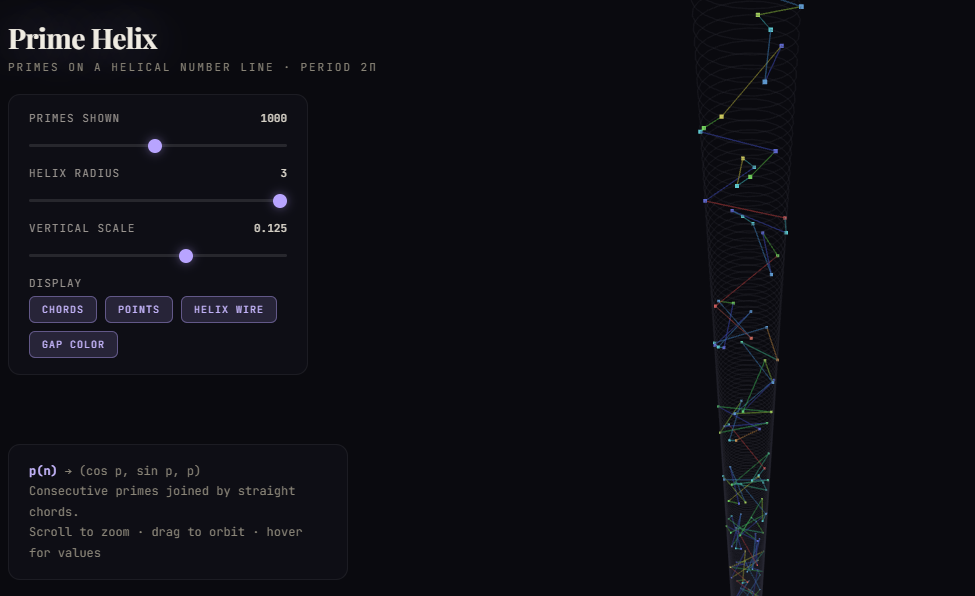
\includegraphics[width=0.82\linewidth]{prime_helix.png}
\caption{The first 1000 primes on the helix $\Hc(t)=(\cos t,\sin t,t)$, joined by chords. Colour indicates the gap to the next prime (violet small, red large). Radius 3 and vertical scale 0.125 for visual clarity.}
\end{figure}

\section{The two-particle experiment}

\subsection{Setup}
Two particles start at $p_1=2$ and move at the same constant speed $v$.
\textbf{Particle A} (the helix walker) follows the helix; after time $T$ it has covered arc length $vT$, an advance of $vT/\sqrt2$ along the number line.
\textbf{Particle B} (the chord hopper) moves only along the chords. After $k$ chords it has covered $D_k=\sum_{n=1}^k d_n$ and reached $p_{k+1}$.

\subsection{The path ratio}
Define the ratio of chord path to helix arc over the same stretch of the number line,
\begin{equation}\label{eq:R}
R(N)=\frac{\sum_{n=1}^{N-1}d_n}{(p_N-p_1)\sqrt2}=\frac{\sum_{n=1}^{N-1}\sqrt{2-2\cos g_n+g_n^2}}{(p_N-2)\sqrt2}.
\end{equation}
For $N=8000$ primes, $R(N)=0.719191$ (Figure~\ref{fig:conv}). The curve is already smooth there, but it is still about $1.7\%$ above its limit $1/\sqrt2\approx0.707107$: the approach is slow, as Section~\ref{sec:fluct} shows. (Version~1 described $R(N)$ as stable to six decimal places at this point. That is true of its local variation, not of its distance to the limit.)

\begin{figure}[ht]
\centering
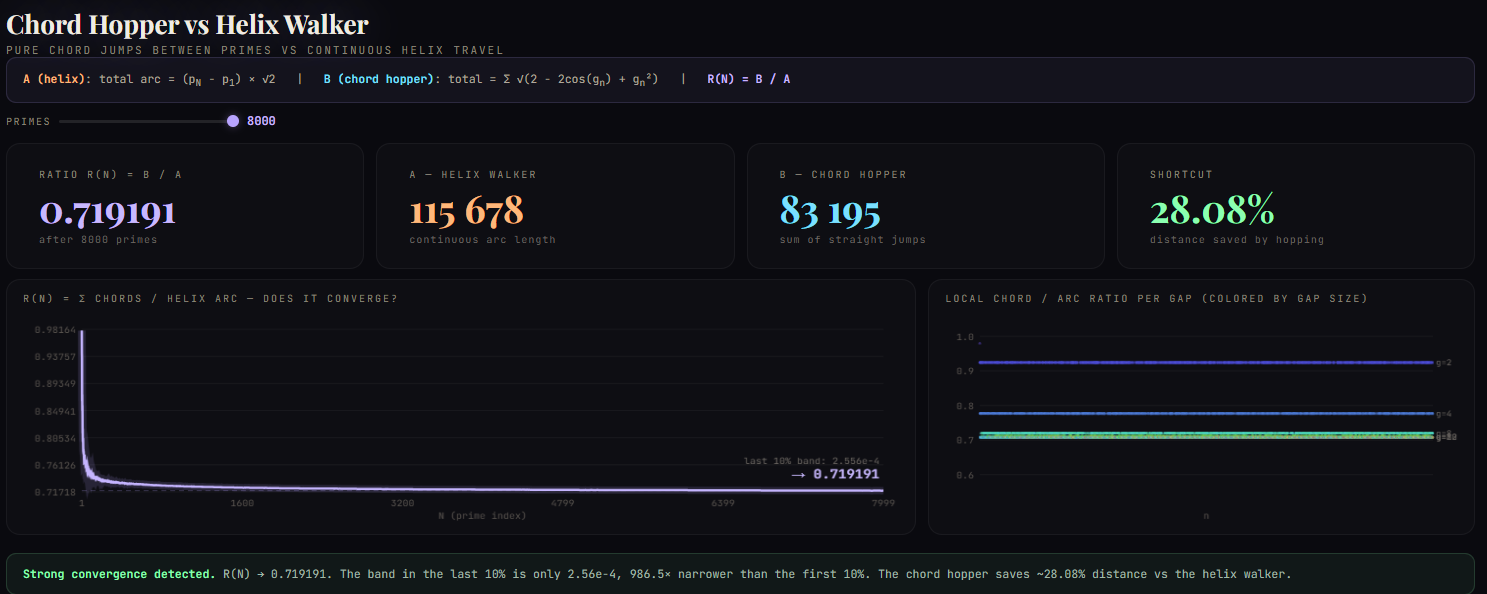
\includegraphics[width=0.95\linewidth]{fig_convergence.png}
\caption{$R(N)$ for the first 8000 primes. Top: cumulative ratio $R(N)\approx0.719$, helix arc, chord path and the $28.08\%$ saved by hopping. Bottom left: $R(N)$ against $N$. Bottom right: local ratio $r_n=d_n/(g_n\sqrt2)$ for each gap, coloured by gap size.}
\label{fig:conv}
\end{figure}

\subsection{The limit and the \texorpdfstring{$45\dg$}{45 degree} pitch}
For a gap $g$ the local ratio is
\begin{equation}\label{eq:local}
r(g)=\frac{\sqrt{g^2+4\sin^2(g/2)}}{g\sqrt2}=\frac1{\sqrt2}+O\!\left(\frac1{g^2}\right),
\end{equation}
because $2-2\cos g=4\sin^2(g/2)\le4$. By the prime number theorem the gaps grow on average like $\ln p_n$, so large gaps dominate the sum and $R(N)\to1/\sqrt2=\cos45\dg$, the cosine of the pitch angle. In the limit the hopper ``cuts out'' the winding and travels almost vertically.

\subsection{The fluctuation term}\label{sec:fluct}
Let $\delta(N)=R(N)-1/\sqrt2$. Since $g+\frac{a}{2g}-\frac{a^2}{8g^3}\le\sqrt{g^2+a}\le g+\frac{a}{2g}$ for $0\le a\le4$, we get with $a=4\sin^2(g/2)$:

\begin{proposition}\label{prop:delta}
\begin{equation}\label{eq:delta}
\delta(N)=\frac{1}{\sqrt2\,(p_N-2)}\sum_{n=1}^{N-1}\left(\frac{2\sin^2(g_n/2)}{g_n}+O\!\left(\frac1{g_n^3}\right)\right),
\end{equation}
and the leading sum is an upper bound for $\delta(N)$.
\end{proposition}

Each gap contributes $O(1/g_n)$, so $\delta(N)$ is a weighted count of small gaps. Twin primes weigh most ($g=2$, $r\approx0.924$); the gap $6$ weighs almost nothing, because $\sin^2 3\approx0.02$. There are about $p_N/\ln p_N$ gaps, and under the Cram\'er--Gallagher heuristic a fixed even gap $g$ occurs with frequency roughly $\mathfrak S(g)/\ln p$, where $\mathfrak S(g)$ is the Hardy--Littlewood singular series \cite{hl,gallagher,granville}. Summing $2\sin^2(g/2)/g$ against these frequencies over $g\lesssim\ln p$ suggests
\begin{equation}\label{eq:rate}
\delta(N)\asymp\frac{a+b\ln\ln p_N}{\ln^2p_N}
\end{equation}
for constants $a,b$ (heuristic, not a theorem). Table~\ref{tab:delta} and Figure~\ref{fig:delta} agree: $\delta(N)\ln^2p_N$ is nearly constant and rises slowly.

\begin{table}[ht]
\centering
\begin{tabular}{rrcccc}
\toprule
$N$ & $p_N$ & $R(N)$ & $\delta(N)$ & $\delta(N)\ln^2p_N$ & $(\ln p_N)^2/\sqrt{p_N}$\\
\midrule
8\,000 & 81\,799 & 0.719191 & 0.01208 & 1.546 & 0.447\\
$10^4$ & 104\,729 & 0.718783 & 0.01168 & 1.560 & 0.413\\
$10^5$ & 1\,299\,709 & 0.715198 & 0.00809 & 1.604 & 0.174\\
$10^6$ & 15\,485\,863 & 0.713114 & 0.00601 & 1.646 & 0.070\\
$5\cdot10^6$ & 86\,028\,121 & 0.712119 & 0.00501 & 1.673 & 0.036\\
\bottomrule
\end{tabular}
\caption{Measured decay of $\delta(N)$. The last column is the rate proposed in version~1; it decays much faster than $\delta(N)$ does.}
\label{tab:delta}
\end{table}

\begin{figure}[ht]
\centering
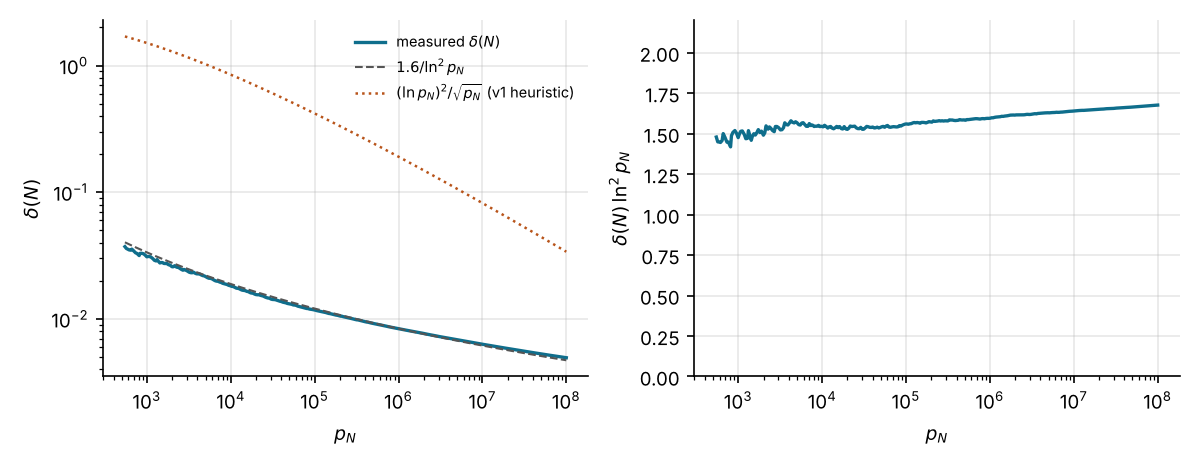
\includegraphics[width=0.95\linewidth]{figures/fig_delta_decay.png}
\caption{Left: $\delta(N)$ against $p_N$, with $1.6/\ln^2p_N$ and the version~1 heuristic $(\ln p_N)^2/\sqrt{p_N}$. Right: $\delta(N)\ln^2p_N$.}
\label{fig:delta}
\end{figure}

\begin{remark}[$\delta(N)$ and the Riemann hypothesis]
Version~1 proposed that $\delta(N)$ decays like $(\ln p_N)^2/\sqrt{p_N}$ if RH holds, and that a zero off the critical line would make it decay more slowly. Both statements should be withdrawn. $\delta(N)$ is dominated by the local average \eqref{eq:delta}, which is of size $1/\ln^2p_N$. Fluctuations of the size that RH controls (relative size about $p^{-1/2}$) are a far smaller, subleading part of $\delta(N)$, invisible beneath the main term. The smoothness of Figure~\ref{fig:conv} therefore says nothing about RH.
\end{remark}

\section{The position ratio}
After time $T$ the helix walker has reached $vT/\sqrt2$ on the number line. The hopper, having covered the same distance $vT$ along chords, has reached approximately
\begin{equation}
\text{position}_B\approx\frac{vT}{\sqrt2}\cdot\frac1{R}\approx vT .
\end{equation}
The hopper advances at effectively $v$, the walker at $v/\sqrt2$. The walker loses the factor $\cos45\dg$ to winding; the hopper, cutting through the inside of the helix, recovers nearly all of it. The part it does not recover is $\delta(N)$: the toll charged by small gaps.

\section{The phasor circle and caustic rings}

\subsection{Projection onto the unit circle}
Projecting the helix onto the $(x,y)$ plane sends $p_n$ to $e^{ip_n}$ on the unit circle, and the chords to chords of the circle. When a few hundred are drawn, concentric rings appear: caustics, the envelopes along which chords of equal angular span concentrate (Figure~\ref{fig:phasor}).

\begin{figure}[ht]
\centering
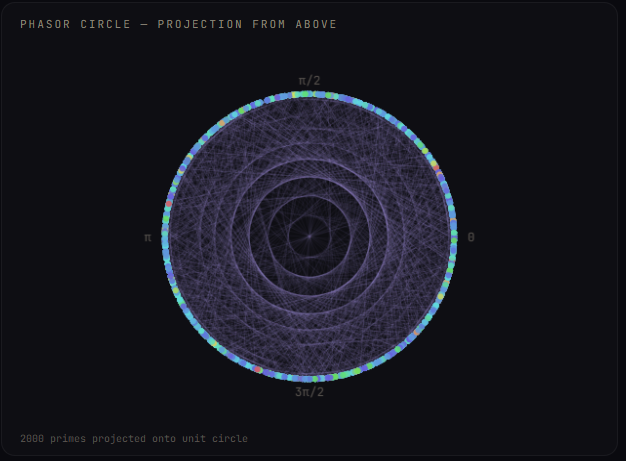
\includegraphics[width=0.6\linewidth]{fig_phasor.png}
\caption{The phasor circle: chords between $e^{ip_n}$ and $e^{ip_{n+1}}$ for 2000 primes. Each ring corresponds to one gap size $g$, at radius $|\cos(g/2)|$.}
\label{fig:phasor}
\end{figure}

\subsection{Caustic radii and gap frequencies}
A chord joining two points of the unit circle at angular separation $\Delta$ is at distance $|\cos(\Delta/2)|$ from the centre, so all chords with the same span are tangent to one circle. With $\Delta=g\bmod2\pi$, gap $g$ produces a caustic of radius
\begin{equation}
r_g=\left|\cos\frac g2\right| .
\end{equation}
(Version~1 omitted the absolute value.) The twin-prime ring has radius $\cos1\approx0.540$. The brightness of a ring grows with the number of consecutive primes with gap $g$. That count is related to, but not the same as, the Hardy--Littlewood singular series $\mathfrak S(g)$, which counts pairs $(p,p+g)$ without requiring them to be consecutive \cite{hl,gallagher}. The chord diagram is in this sense an optical histogram of gaps.

\section{The prime phase function}
Define $\theta(n)=p_n\bmod2\pi$. Because $1/(2\pi)$ is irrational, $\theta(n)$ is equidistributed on $[0,2\pi)$. For the primes this is Vinogradov's theorem \cite{vinogradov}; Weyl's theorem \cite{weyl} covers $n\alpha$ for all integers $n$, not the primes. In 12 bins of the circle, primes up to $10^7$ fill each bin to within $1.6\%$ of the mean.

\begin{figure}[ht]
\centering
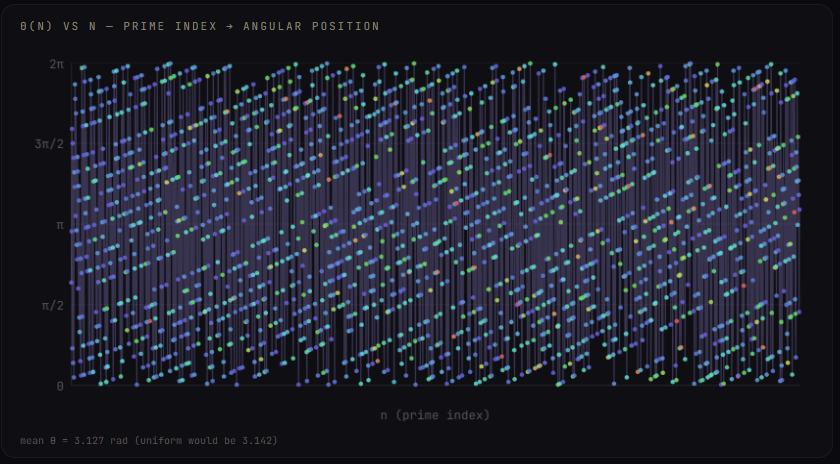
\includegraphics[width=0.95\linewidth]{fig_theta.png}
\caption{$\theta(n)=p_n\bmod2\pi$ against the prime index $n$ for 2000 primes. Diagonal striations come from runs of similar gaps; vertical drops mark large gaps where the phase wraps round several times.}
\label{fig:theta}
\end{figure}

When $\theta(n)$ is plotted against $n$ (Figure~\ref{fig:theta}), diagonal striations appear. A run of gaps of size $g$ produces a line of slope $g\bmod2\pi$ per index, and the common gaps $2$, $4$, $6$ dominate. The figure is thus a picture of the local gap sequence.

\begin{remark}[Correction to version~1]
Version~1 interpreted the striations as the oscillations of the explicit formula and predicted that a Fourier analysis of $\theta(n)$ would show peaks at the zeros of $\zeta$. That cannot work. The zero $\rho=\frac12+i\gamma$ enters prime sums through $p^{-i\gamma}=e^{-i\gamma\ln p}$, a winding that is logarithmic in $p$. The helix winds linearly, $e^{ip}$, and sums such as $\sum e^{ip}$ are exponential sums over primes of the kind estimated by Vinogradov's method; they do not single out the zeros of $\zeta$. Section~\ref{sec:zeros} gives the helical picture in which the zeros do appear.
\end{remark}

\section{Chord shapes and the screw symmetry}\label{sec:chords}

\subsection{One shape per gap}
Consider the general helix $\Hc_{r,\omega,c}(t)=(r\cos\omega t,\ r\sin\omega t,\ ct)$. The screw motions $S_\tau$, a rotation by $\omega\tau$ about the axis combined with a translation by $c\tau$ along it, map the helix to itself: $S_\tau\Hc(t)=\Hc(t+\tau)$.

\begin{proposition}\label{prop:screw}
The chord from $\Hc(p)$ to $\Hc(p+g)$ is the image under $S_p$ of the chord from $\Hc(0)$ to $\Hc(g)$. Hence its length and its tilt against the horizontal,
\begin{equation}
L(g)=\sqrt{4r^2\sin^2(\omega g/2)+c^2g^2},\qquad \tan\alpha(g)=\frac{c\,g}{2r\,|\sin(\omega g/2)|},
\end{equation}
depend on $g$ only, and the whole chain of chords $\Hc(p_1)\to\Hc(p_2)\to\cdots$ is determined, up to the screw motion $S_{p_1}$, by the gap sequence $(g_n)$. In particular the angle $\phi_n$ between consecutive chords satisfies
\begin{equation}\label{eq:turn}
\cos\phi_n=\frac{4r^2\sin\frac{\omega g_n}2\sin\frac{\omega g_{n+1}}2\cos\frac{\omega(g_n+g_{n+1})}2+c^2g_ng_{n+1}}{L(g_n)\,L(g_{n+1})},
\end{equation}
a function of the pair $(g_n,g_{n+1})$ alone.
\end{proposition}

\begin{proof}
$S_p$ is an isometry with $S_p\Hc(0)=\Hc(p)$ and $S_p\Hc(g)=\Hc(p+g)$. Translating the chain so that $p_1$ sits at $0$ is one screw motion, after which every point is $\Hc(p_1+g_1+\dots+g_k)$. For \eqref{eq:turn}, write the horizontal part of the chord from angle $a$ to angle $b$ as $2r\sin\frac{b-a}2\,\big(-\sin\frac{a+b}2,\cos\frac{a+b}2\big)$ and take the dot product of consecutive chords.
\end{proof}

\begin{remark}[Where the uniqueness comes from]
Every chord is a different vector in space, because its orientation about the axis, $\omega(p+g/2)$, differs from chord to chord. That uniqueness comes from $\omega/2\pi$ being irrational, and it holds for any sequence of distinct integers on the helix. It is not a property of the primes. What is specific to the primes is which gaps occur and how often, and in which order.
\end{remark}

For primes $5\le p\le10^7$ there are 664\,576 chords but only 74 distinct shapes $(L,\alpha)$, exactly one for each gap value that occurs. The geometry of the chain is therefore a faithful picture of the gap sequence, and every statistic of the chain is a statistic of gaps.

\subsection{Comparison with random models}
To see which features of the chain are specific to the primes, we compare it with two random models on $(10^3,10^7]$:
\begin{itemize}[nosep]
\item \textbf{Cram\'er's model} \cite{cramer}: each $n$ is ``prime'' independently with probability $1/\ln n$.
\item \textbf{Granville's refinement} \cite{granville}: only $n$ coprime to $W=\prod_{q\le z}q$ are allowed, each with probability $\frac{W}{\varphi(W)}\cdot\frac1{\ln n}$. This builds in sieving by the primes up to $z$; we use $z=7$ and $z=13$.
\end{itemize}

\begin{figure}[ht]
\centering
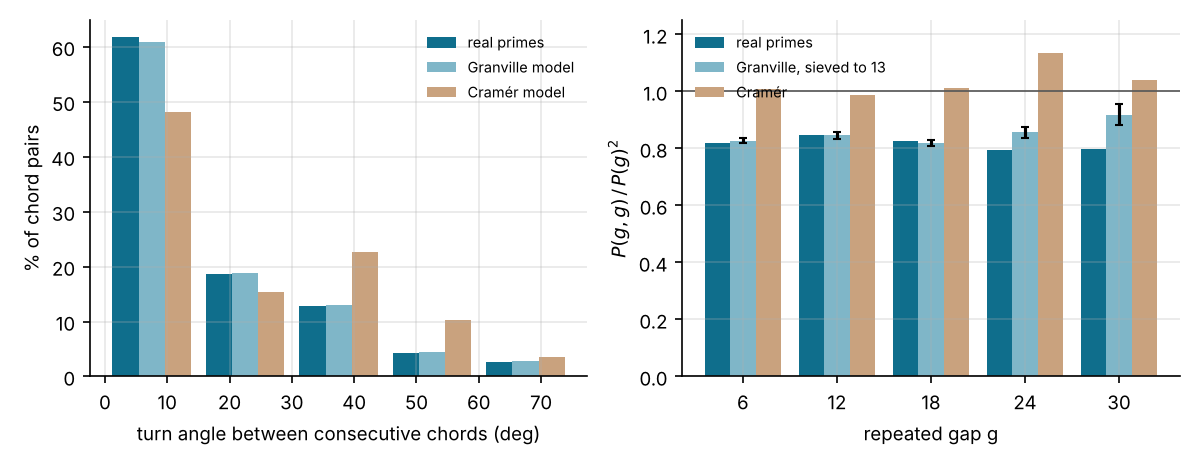
\includegraphics[width=0.95\linewidth]{figures/fig_turn_repeats.png}
\caption{Left: turn angle $\phi_n$ between consecutive chords on $\Hc(t)=(\cos t,\sin t,t)$, for the primes and both models. Right: how often a gap is immediately repeated, relative to independent gaps, $P(g,g)/P(g)^2$; Granville's model is the mean and standard deviation of 8 runs.}
\label{fig:turn}
\end{figure}

\begin{table}[ht]
\centering
\small\setlength{\tabcolsep}{4pt}
\begin{tabular}{lccccc}
\toprule
$g$ & 6 & 12 & 18 & 24 & 30\\
\midrule
Primes & 0.818 & 0.848 & 0.825 & 0.796 & 0.798\\
Granville, $z=13$ & $0.827\pm0.008$ & $0.846\pm0.011$ & $0.820\pm0.010$ & $0.857\pm0.020$ & $0.919\pm0.036$\\
Granville, $z=7$ & $0.831\pm0.007$ & $0.885\pm0.011$ & $0.855\pm0.010$ & $0.844\pm0.031$ & $0.956\pm0.029$\\
Cram\'er (1 run) & 1.010 & 0.988 & 1.012 & 1.135 & 1.039\\
\bottomrule
\end{tabular}
\caption{Repeated gaps, $P(g_n=g_{n+1}=g)/P(g)^2$, for primes and models on $(10^3,10^7]$. The pairs $(2,2)$ and $(4,4)$ never occur among primes above $7$, since one of the three numbers would be divisible by $3$.}
\label{tab:repeat}
\end{table}

Three observations follow (Figure~\ref{fig:turn}, Table~\ref{tab:repeat}).
\begin{enumerate}[nosep]
\item Cram\'er's model gets the chain wrong from the start: about half its gaps are odd, and its turn-angle distribution differs visibly from that of the primes.
\item Granville's model reproduces the turn-angle distribution of the primes to within about one percentage point in every bin, and reproduces the avoidance of repeated gaps $6$, $12$, $18$. These features are explained by sieving with small primes.
\item For the repeated gaps $24$ and $30$ the primes avoid repetition more strongly than the model, by about three standard deviations of the model runs. Raising $z$ from $7$ to $13$ narrowed the difference for $g=30$ but not for $g=24$, so this test cannot yet separate further sieving effects from the bias between consecutive primes found by Lemke Oliver and Soundararajan \cite{los}, who explain it through the second-order terms of the Hardy--Littlewood conjectures.
\end{enumerate}
The sequence of turn angles of the chord chain is thus a geometric way of seeing a known and genuinely subtle phenomenon. We make no claim of a new effect.

\section{Connection to the prime number theorem}
The prime number theorem \cite{hadamard,vallee},
\begin{equation}
\pi(x)\sim\frac{x}{\ln x},
\end{equation}
says that the average gap near $x$ grows like $\ln x$. By \eqref{eq:local} each local ratio is $1/\sqrt2+O(1/g_n^2)$, and these corrections vanish in the cumulative average as gaps grow; Proposition~\ref{prop:delta} gives the rate. In geometric language: \emph{the prime number theorem says that, on the helix, the chord hopper eventually stops feeling the curvature of $e^{i\theta}$.}

\section{Where the zeros live: the logarithmic winding}\label{sec:zeros}

\subsection{The explicit formula}
The link between primes and zeros is the explicit formula of Riemann and von Mangoldt \cite{riemann,mangoldt,davenport}:
\begin{equation}
\psi(x)=x-\sum_\rho\frac{x^\rho}{\rho}-\ln(2\pi)-\frac12\ln\!\left(1-\frac1{x^2}\right),
\end{equation}
where $\psi(x)=\sum_{p^k\le x}\ln p$ and $\rho$ runs over the nontrivial zeros. A zero $\rho=\frac12+i\gamma$ contributes $x^{1/2}\cos(\gamma\ln x-\varphi_\rho)$ up to its amplitude: a wave in $\ln x$. This is the ``music of the primes'' \cite{dusautoy,berrykeating}.

\subsection{Linear versus logarithmic winding}
The helix of this paper winds once per $2\pi$ units of $p$. A zero winds once per factor $e^{2\pi/\gamma}$ of $p$; for $\gamma_1=14.1347\ldots$ that is a factor of about $1.56$. The natural helix for the zeros is therefore one that winds in $\ln p$: we place the prime power $n$ at angle $-t\ln n$ and give it weight $\Lambda(n)/\sqrt n$, which places the walk on the critical line $s=\frac12+it$.

\begin{definition}
For $t>0$ and $N\ge2$ let
\begin{equation}\label{eq:walk}
W_t(N)=\sum_{n\le N}\frac{\Lambda(n)}{\sqrt n}\,e^{-it\ln n}-\frac{N^{1/2-it}-1}{1/2-it},
\end{equation}
the partial sums of $\sum\Lambda(n)n^{-s}$ at $s=\frac12+it$, with the contribution $\int_1^Nx^{-s}\,dx$ of the pole of $\zeta$ at $s=1$ removed.
\end{definition}

Without the subtraction, the pole produces a spiral of radius about $\sqrt N/t$ that hides everything else.

\subsection{The walk near a zero}
Formally applying the explicit formula for $\sum_{n\le N}\Lambda(n)n^{-s}$ (see \cite[ch.~17]{davenport}, \cite[\S5.5]{ik}) gives
\begin{equation}
W_t(N)\approx C(s)-\sum_\rho\frac{N^{\rho-s}}{\rho-s},
\end{equation}
with $C(s)$ independent of $N$. If $t$ is near a zero, write $\rho-s=i(\gamma-t)$. The term of that zero is $\frac{i}{\gamma-t}N^{i(\gamma-t)}$: as $N$ grows it runs round a circle of radius $1/|\gamma-t|$, and combined with the pole of $-\zeta'/\zeta$ at $\rho$ in $C(s)$ the circle passes through the starting point $W=0$. As $t\to\gamma$ the circle opens into the straight line $W_\gamma(N)\approx-\ln N$. This is a heuristic (the sum over zeros converges only conditionally), confirmed numerically: for $N=10^5$ ($-\ln N=-11.51$),
\[
W_{\gamma_1}(10^5)=-10.89+0.18i,\qquad\max_{n\le10^5}|W_{15}(n)|=3.12 ,
\]
the second value being close to the predicted circle diameter $2/|15-\gamma_1|=2.31$ plus the scatter from the other zeros (Figure~\ref{fig:walk}).

\begin{figure}[ht]
\centering
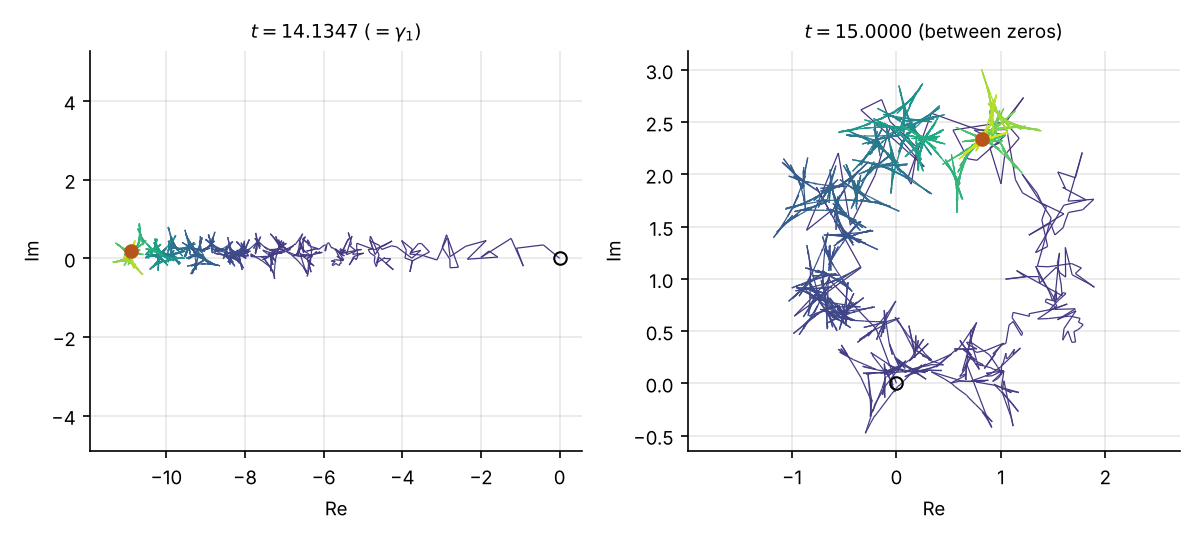
\includegraphics[width=0.95\linewidth]{figures/fig_log_walk.png}
\caption{The logarithmic walk $W_t(n)$, $n\le10^5$, at the first zero $t=\gamma_1$ (left) and between zeros at $t=15$ (right). Ring: start; dot: end; colour from small to large $n$.}
\label{fig:walk}
\end{figure}

\subsection{The resonance spectrum}
To see all the zeros at once we use a smooth cutoff and remove the pole term in closed form:
\begin{equation}
H_X(t)=\sum_{n\le X}\Big(1-\frac nX\Big)^2\frac{\Lambda(n)}{\sqrt n}e^{-it\ln n}-\int_1^X\Big(1-\frac xX\Big)^2x^{-1/2-it}\,dx .
\end{equation}
For $X=2\cdot10^6$ the peaks of $|H_X(t)|$ on $8\le t\le50$ fall at the zeros (Figure~\ref{fig:spec}, Table~\ref{tab:peaks}).

\begin{table}[ht]
\centering
\resizebox{\linewidth}{!}{%
\begin{tabular}{l*{10}{c}}
\toprule
Peak of $|H_X|$ & 14.14 & 21.02 & 25.02 & 30.42 & 32.94 & 37.58 & 40.91 & 43.34 & 47.98 & 49.79\\
Zero $\gamma$ & 14.135 & 21.022 & 25.011 & 30.425 & 32.935 & 37.586 & 40.919 & 43.327 & 48.005 & 49.774\\
\bottomrule
\end{tabular}}
\caption{Peaks of the smoothed logarithmic walk against the zeros of $\zeta$ (zeros from Odlyzko's tables \cite{odlyzko}). Grid step $0.01$.}
\label{tab:peaks}
\end{table}

\begin{figure}[ht]
\centering
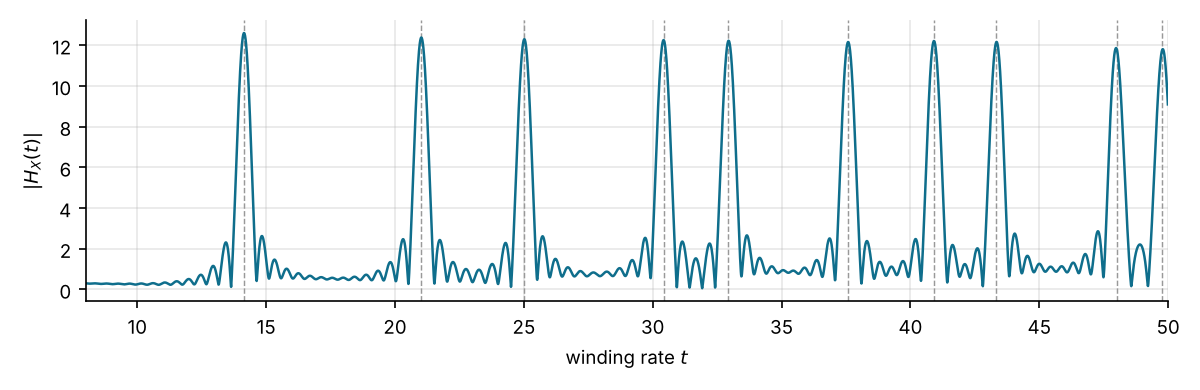
\includegraphics[width=0.95\linewidth]{figures/fig_log_spectrum.png}
\caption{$|H_X(t)|$ for $X=2\cdot10^6$. Dashed lines: the first ten zeros of $\zeta$.}
\label{fig:spec}
\end{figure}

\begin{remark}[The dual picture]
The reverse direction also holds. Landau's formula \cite{landau} states that for fixed $x>1$, $\sum_{0<\gamma\le T}x^\rho=-\frac{T}{2\pi}\Lambda(x)+O(\ln T)$. Summing waves over the zeros therefore produces spikes at the prime powers, with heights $\ln p/p^{k/2}$ if RH holds. A walk over primes resonates at the zeros; a walk over zeros resonates at the primes. None of this is new: it is the explicit formula. What the helix adds is a picture of it.
\end{remark}

\section{Analogies, clearly labelled}
Version~1 drew three further parallels. We keep them as analogies only, and say why none of them is a mathematical correspondence.
\begin{itemize}[nosep]
\item \textbf{Euler product.} The smooth helix arc and the sum of chords resemble the two sides of $\sum n^{-s}=\prod_p(1-p^{-s})^{-1}$. But $R(N)$ uses only the gap sequence, while the Euler product encodes multiplicative structure. Any increasing sequence with gaps growing on average gives the same limit.
\item \textbf{The $45\dg$ pitch and the pole at $s=1$.} Both fix a leading-order behaviour. But changing the pitch to $(\cos t,\sin t,\beta t)$ changes the limit to $\cos\arctan(1/\beta)$ trivially, while the pole of $\zeta$ is a property of the integers.
\item \textbf{The $45\dg$ balance and the critical line.} On the helix, climb equals winding at $45\dg$; the critical line is $\operatorname{Re}s=\frac12$. The critical line concerns where the zeros lie; it has no geometric relation to the pitch of this helix.
\end{itemize}

\section{Geometric invariance}
The limit $R(N)\to1/\sqrt2$ is set by the pitch of the helix and the growth of gaps, not by the arithmetic of the primes. Any sequence with gaps growing on average gives the same limit. We may call this geometric invariance: the large-scale statistics of prime spacing pass through this embedding unchanged. The finer structure, in $\delta(N)$ and in the order of gaps, is where primes and random sequences differ, and Sections~\ref{sec:fluct} and \ref{sec:chords} make that difference measurable.

\section{Correspondence between constructions}

\begin{table}[ht]
\centering
\small
\begin{tabular}{>{\raggedright}p{4.4cm}>{\raggedright}p{5.6cm}p{2.9cm}}
\toprule
Helical construction & Classical counterpart & Status\\
\midrule
$R(N)\to1/\sqrt2$ & Prime number theorem & Follows from PNT\\
$\delta(N)\asymp1/\ln^2p_N$ & Small-gap frequencies (Hardy--Littlewood) & Heuristic, numerical\\
Caustic rings & Gap histogram; related to $\mathfrak S(g)$ & Geometric fact\\
Chord chain up to screw motion & Gap sequence $(g_n)$ & Proposition~\ref{prop:screw}\\
Turn angles, repeated shapes & Consecutive-gap statistics; Lemke Oliver--Soundararajan bias & Numerical\\
Striations in $\theta(n)$ & Runs of similar gaps & Geometric fact\\
Equidistribution of $\theta(n)$ & Vinogradov's theorem & Theorem\\
Resonances of the log walk $W_t$ & Zeros of $\zeta$ via the explicit formula & Known; numerical\\
$45\dg$ pitch; arc vs.\ chords & Pole at $s=1$; Euler product & Analogy only\\
\bottomrule
\end{tabular}
\caption{Helical construction and classical theory, with the status of each correspondence.}
\end{table}

\section{Discussion and future directions}
The construction proves no new theorem about primes. Its value is translation: it renders the prime number theorem, gap statistics and the explicit formula in a geometric and kinematic language accessible without complex analysis. A student who understands helices, particles and chord lengths can \emph{see} what the zeta function \emph{computes}.

Directions that remain open:
\begin{enumerate}[nosep]
\item \textbf{The constants in \eqref{eq:rate}.} Derive $a$ and $b$ from the Hardy--Littlewood singular series and compare with $\delta(N)\ln^2p_N\approx1.55$--$1.67$.
\item \textbf{Caustic brightness.} Measure ring brightness as a function of $g$ and compare with the predicted frequencies of consecutive gaps.
\item \textbf{Repeated shapes.} Extend Table~\ref{tab:repeat} beyond $10^7$ and to larger $z$, to separate sieving effects from the Lemke Oliver--Soundararajan bias.
\item \textbf{Two helices.} Present the linear helix (gaps) and the logarithmic helix (zeros) side by side, as the two halves of the explicit formula.
\item \textbf{Other sequences.} Apply the construction to semiprimes, prime constellations and primes in arithmetic progressions.
\end{enumerate}

\section{Conclusion}
Euler's formula, read in three dimensions, is a helix. Primes placed on it and joined by chords make a chain whose shape is a faithful picture of the gap sequence. The two-particle ratio tends to $\cos45\dg$ by the prime number theorem, and its deviation measures small gaps, decaying like $1/\ln^2p_N$. The order of the chords shows the tendency of consecutive primes not to repeat a gap. The zeros of $\zeta$ do not live on this helix but on its logarithmic counterpart, where a walk over prime powers resonates at $14.1347\ldots$, $21.0220\ldots$ and the rest. We hope the helix is a useful way to look at an old problem from a different angle, and an honest one.

\section*{Acknowledgements}
The numerical checks and revisions in version~2 were prepared with the help of Claude (Anthropic). Every number is reproduced by \texttt{analysis/prime\_helix\_checks.py}.

\appendix
\section{Changes from version 1}\label{app:rev}
\begin{enumerate}[nosep]
\item Section~3.2: $R(8000)$ is smooth but $1.7\%$ above its limit; ``stable to six decimal places'' rephrased.
\item Section~3.4: new Proposition~\ref{prop:delta}, measured rate $\delta(N)\asymp1/\ln^2p_N$ (Table~\ref{tab:delta}); the RH rate $(\ln p_N)^2/\sqrt{p_N}$ and the claimed link between $\delta(N)$ and RH withdrawn. The form $c/\ln p_N$ proposed in version~1 replaced.
\item Section~5: caustic radius $|\cos(g/2)|$; ring brightness distinguished from $\mathfrak S(g)$.
\item Section~6: equidistribution of $p_n\bmod2\pi$ attributed to Vinogradov, not Weyl; interpretation of striations as zeta-zero oscillations and the predicted Fourier peaks withdrawn.
\item New Section~7: screw symmetry, one shape per gap, comparison with Cram\'er and Granville models.
\item New Section~9: logarithmic winding, walk $W_t(N)$, resonance spectrum, Landau's formula. Replaces Sections~10.3--10.5 of version~1.
\item Section~10: Euler product, pole and critical-line parallels kept as labelled analogies; Table~1 gains a status column.
\item Degree signs restored ($45\dg$ was printed as ``45'').
\item References: Bombieri's asymptotic sieve and Goldston--Pintz--Y{\i}ld{\i}r{\i}m removed (not supporting the cited claims); Vinogradov, Cram\'er, Gallagher, Granville, Lemke Oliver--Soundararajan, Landau, Iwaniec--Kowalski and Odlyzko added.
\end{enumerate}

\begin{thebibliography}{99}\small
\bibitem{ahlfors} L.~V. Ahlfors, \emph{Complex Analysis}, 3rd ed., McGraw-Hill, 1979.
\bibitem{needham} T.~Needham, \emph{Visual Complex Analysis}, Oxford University Press, 1997.
\bibitem{weylRS} H.~Weyl, \emph{The Concept of a Riemann Surface}, Addison-Wesley, 1955 (original 1913).
\bibitem{riemann} B.~Riemann, Ueber die Anzahl der Primzahlen unter einer gegebenen Gr\"osse, \emph{Monatsber. Berliner Akad.}, 1859.
\bibitem{hadamard} J.~Hadamard, Sur la distribution des z\'eros de la fonction $\zeta(s)$ et ses cons\'equences arithm\'etiques, \emph{Bull. Soc. Math. France} 24 (1896), 199--220.
\bibitem{vallee} C.-J. de la Vall\'ee Poussin, Recherches analytiques sur la th\'eorie des nombres premiers, \emph{Ann. Soc. Sci. Bruxelles} 20 (1896), 183--256.
\bibitem{mangoldt} H.~von Mangoldt, Zu Riemanns Abhandlung ``Ueber die Anzahl der Primzahlen unter einer gegebenen Gr\"osse'', \emph{J. reine angew. Math.} 114 (1895), 255--305.
\bibitem{landau} E.~Landau, \"Uber die Nullstellen der Zetafunktion, \emph{Math. Ann.} 71 (1911), 548--564.
\bibitem{weyl} H.~Weyl, \"Uber die Gleichverteilung von Zahlen mod.\ Eins, \emph{Math. Ann.} 77 (1916), 313--352.
\bibitem{hl} G.~H. Hardy and J.~E. Littlewood, Some problems of `Partitio numerorum'; III: On the expression of a number as a sum of primes, \emph{Acta Math.} 44 (1923), 1--70.
\bibitem{cramer} H.~Cram\'er, On the order of magnitude of the difference between consecutive prime numbers, \emph{Acta Arith.} 2 (1936), 23--46.
\bibitem{vinogradov} I.~M. Vinogradov, \emph{The Method of Trigonometric Sums in the Theory of Numbers}, Interscience, 1954.
\bibitem{gallagher} P.~X. Gallagher, On the distribution of primes in short intervals, \emph{Mathematika} 23 (1976), 4--9.
\bibitem{granville} A.~Granville, Harald Cram\'er and the distribution of prime numbers, \emph{Scand. Actuarial J.} 1995(1), 12--28.
\bibitem{berrykeating} M.~V. Berry and J.~P. Keating, The Riemann zeros and eigenvalue asymptotics, \emph{SIAM Review} 41 (1999), 236--266.
\bibitem{davenport} H.~Davenport, \emph{Multiplicative Number Theory}, 3rd ed., revised by H.~L. Montgomery, Springer GTM 74, 2000.
\bibitem{dusautoy} M.~du Sautoy, \emph{The Music of the Primes}, HarperCollins, 2003.
\bibitem{ik} H.~Iwaniec and E.~Kowalski, \emph{Analytic Number Theory}, AMS Colloquium Publications 53, 2004.
\bibitem{los} R.~J. Lemke Oliver and K.~Soundararajan, Unexpected biases in the distribution of consecutive primes, \emph{Proc. Natl. Acad. Sci. USA} 113 (2016), E4446--E4454.
\bibitem{odlyzko} A.~M. Odlyzko, Tables of zeros of the Riemann zeta function, \url{https://www-users.cse.umn.edu/~odlyzko/zeta_tables/}.
\end{thebibliography}

\end{document}
